%%%%%%%%%%%%%%%%%%%%%%%%%%%%%%%%%%%%%%%%%%%%%%%%%%%%%%%%%%%%%%%%%%%%%
%
% CSCI 1430 Writeup Template
%
% This is a LaTeX document. LaTeX is a markup language for producing 
% documents. Your task is to fill out this
% document, then to compile this into a PDF document. 
% You will then upload this PDF to `Gradescope' - the grading system 
% that we use.
%
% 
% TO COMPILE:
% > pdflatex thisfile.tex
%
% For references to appear correctly instead of as '??', you must run 
% pdflatex twice.
%
% If you do not have LaTeX and need a LaTeX distribution:
% - Departmental machines have one installed.
% - Personal laptops (all common OS): www.latex-project.org/get/
%
% If you need help with LaTeX, please come to office hours. 
% Or, there is plenty of help online:
% https://en.wikibooks.org/wiki/LaTeX
%
% Good luck!
% James and the 1430 staff
%
%%%%%%%%%%%%%%%%%%%%%%%%%%%%%%%%%%%%%%%%%%%%%%%%%%%%%%%%%%%%%%%%%%%%%
%
% How to include two graphics on the same line:
% 
% \includegraphics[\width=0.49\linewidth]{yourgraphic1.png}
% \includegraphics[\width=0.49\linewidth]{yourgraphic2.png}
%
% How to include equations:
%
% \begin{equation}
% y = mx+c
% \end{equation}
% 
%%%%%%%%%%%%%%%%%%%%%%%%%%%%%%%%%%%%%%%%%%%%%%%%%%%%%%%%%%%%%%%%%%%%%%%%%%%%%%%%%%%%%%%%%%%%%%%%

\documentclass[11pt]{article}

\usepackage[english]{babel}
\usepackage[utf8]{inputenc}
\usepackage[colorlinks = true,
            linkcolor = blue,
            urlcolor  = blue]{hyperref}
\usepackage[a4paper,margin=1.5in]{geometry}
\usepackage{stackengine,graphicx}
\usepackage{fancyhdr}
\setlength{\headheight}{15pt}
\usepackage{microtype}
\usepackage{times}
\usepackage{booktabs}

% From https://ctan.org/pkg/matlab-prettifier
\usepackage[numbered,framed]{matlab-prettifier}

\frenchspacing
\setlength{\parindent}{0cm} % Default is 15pt.
\setlength{\parskip}{0.3cm plus1mm minus1mm}

\pagestyle{fancy}
\fancyhf{}
\lhead{Project Writeup}
\rhead{CS172}
\rfoot{\thepage}

\title{\vspace{-1cm}Project 1 Writeup}
\author{No one}
\date{\today}


\begin{document}
\maketitle
\vspace{-1.5cm}
\thispagestyle{fancy}

\section*{Data Processing}
	In 1-D convolution, we need to extend two arrays operated on. We can extend with zeros or something else depending on kinds of convolutions. Hence, we also have to preprocess matrices before we convolve them. We have several choices to do it, 'circular', 'replicate', 'symmetric'. According to the requirements, we use zero padding and symmetric padding to process image matrices and we will talk about their different.

\section{Algorithm}
	\subsection{2D Convolution in Spacial Domain}
	After padding the image matrix, for every pixel of the image, we select a sub-matrix whose center is the current pixel and the size of the matrix is the same as the filter matrix. Multiply them by every corresponding element with that the center of the filter matrix has to be multiplied with the current pixel and take the sum of products. The sum is the color value of the corresponding pixel. If the image is presented as RGB, we could do the same operation in three channels at the same time. 
	\begin{figure}[h]
		\centering
		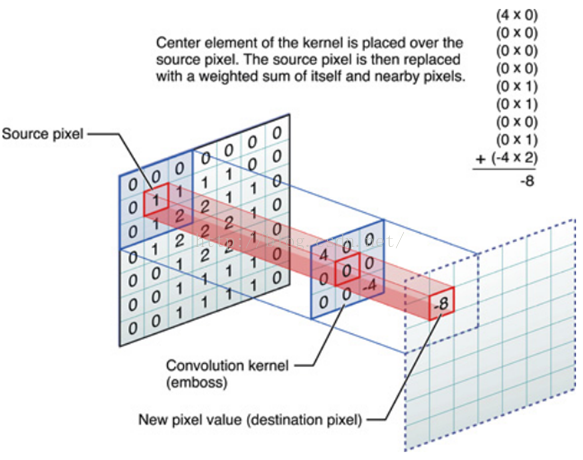
\includegraphics[width=8cm]{convolution}
		\caption{2D convolution in one channel}
	\end{figure}
	
	\subsection{2D Convolution in Frequency Domain}
	In the Frequency Domain, the convolution operation becomes a multiplication instead, which is faster. In the Frequency Domain, we can use the Fast Fourier Transform to transform the image matrix and filter matrix, then we multiply their transform. Eventually, we use the Inverse Fast Fourier Transform on the product and then we choose the effective part as the output. Moreover, we also need to preprocess the two matrix so that we can easily find the result. 

\section{Result}
Here are the result of aligned images provided and I also find one pair of aligned image and hybrid them.
\subsection{Cat and Dog}
\begin{figure}[h]
	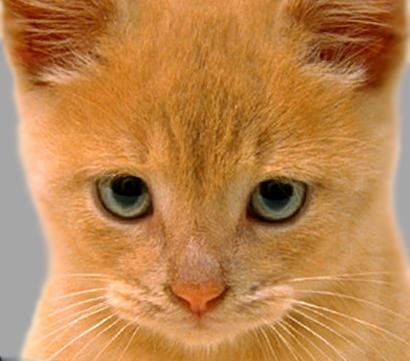
\includegraphics[width=5cm]{cat.jpg}
	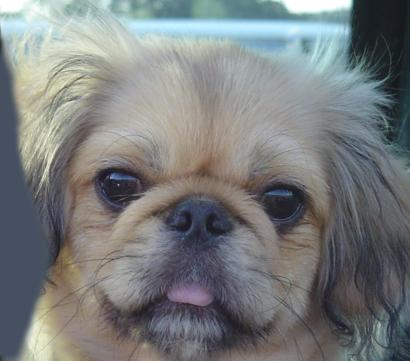
\includegraphics[width=5cm]{dog.jpg}\\
	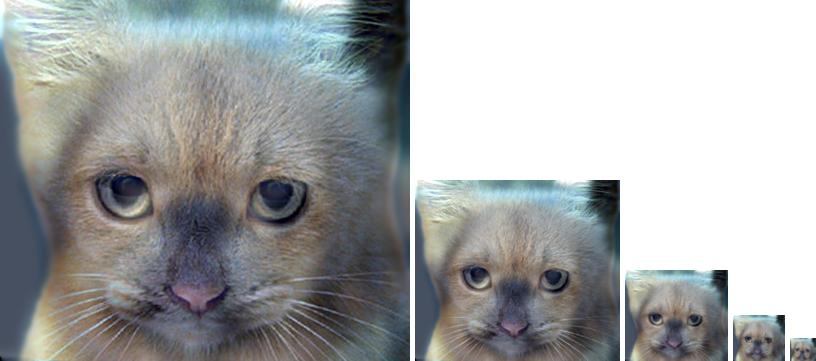
\includegraphics[width=10cm]{hybrid1.jpg}
	\caption{hybrid image 1}
\end{figure}
\newpage
\subsection{Plane and Bird}
\begin{figure}[h]
	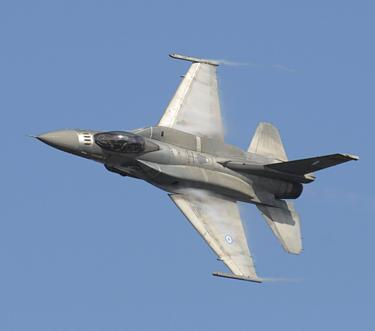
\includegraphics[width=5cm]{plane.jpg}
	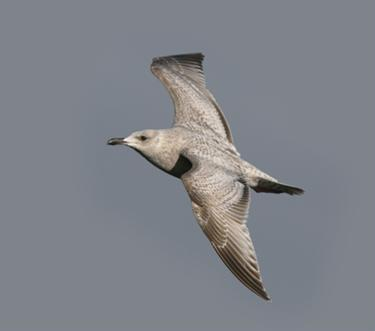
\includegraphics[width=5cm]{bird.jpg}\\
	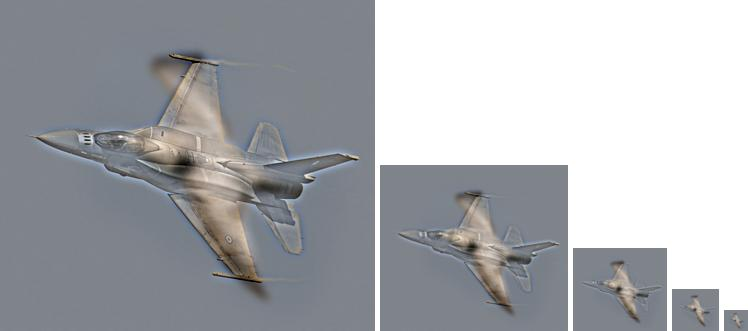
\includegraphics[width=10cm]{hybrid2.jpg}
	\caption{hybrid image 2}
\end{figure}
\newpage
\subsection{Marilyn and Einstein}
\begin{figure}[h]
	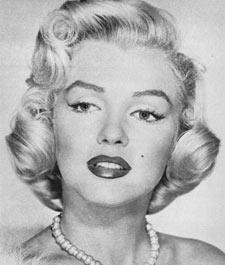
\includegraphics[width=5cm]{marilyn.jpg}
	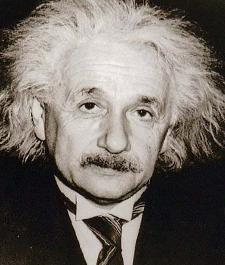
\includegraphics[width=5cm]{einstein.jpg}\\
	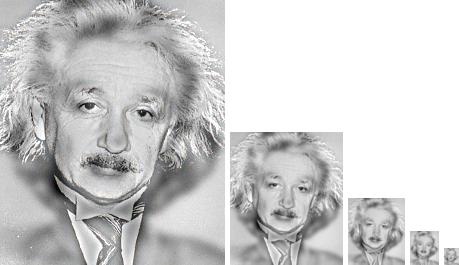
\includegraphics[width=10cm]{hybrid3.jpg}
	\caption{hybrid image 3}
\end{figure}
\newpage
\subsection{Bicycle and Motorcycle}
\begin{figure}[h]
	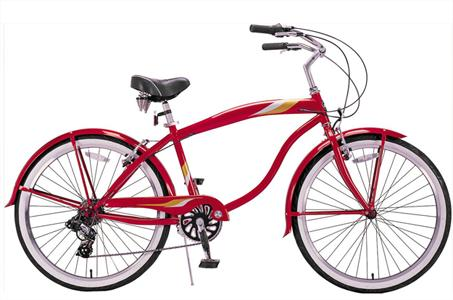
\includegraphics[width=5cm]{bicycle.jpg}
	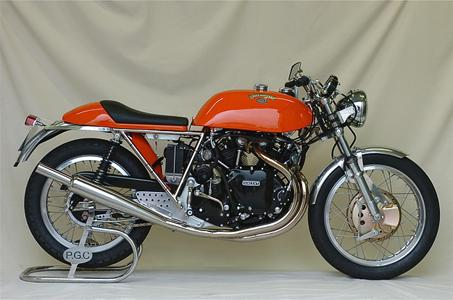
\includegraphics[width=5cm]{motorcycle.jpg}\\
	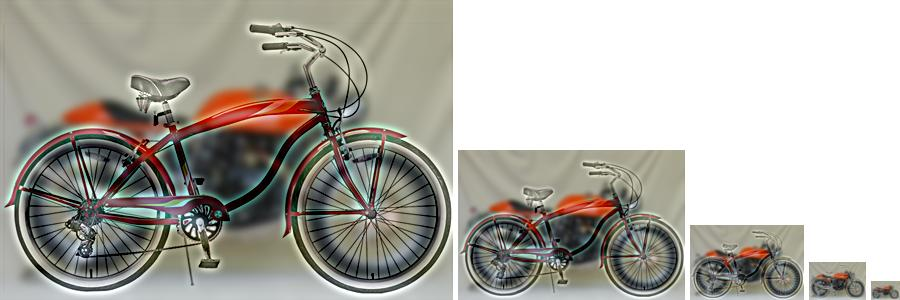
\includegraphics[width=10cm]{hybrid4.jpg}
	\caption{hybrid image 4}
\end{figure}
\newpage
\subsection{Fish and Submarine}
\begin{figure}[h]
	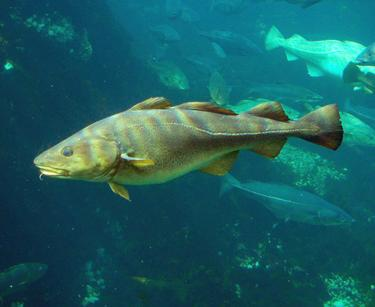
\includegraphics[width=5cm]{fish.jpg}
	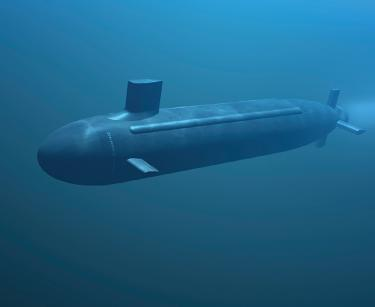
\includegraphics[width=5cm]{submarine.jpg}\\
	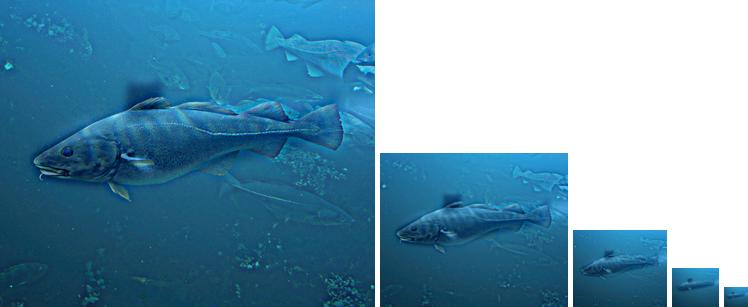
\includegraphics[width=10cm]{hybrid5.jpg}
	\caption{hybrid image 5}
\end{figure}
\newpage
\subsection{James and Wade}
\begin{figure}[h]
	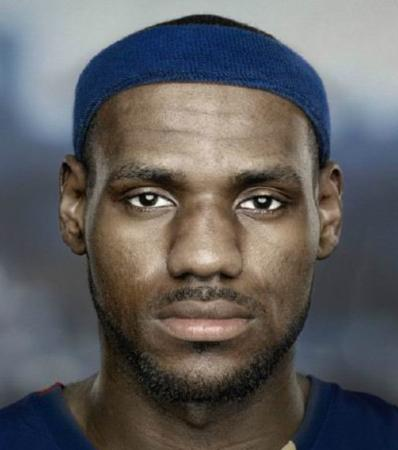
\includegraphics[width=5cm]{james.jpg}
	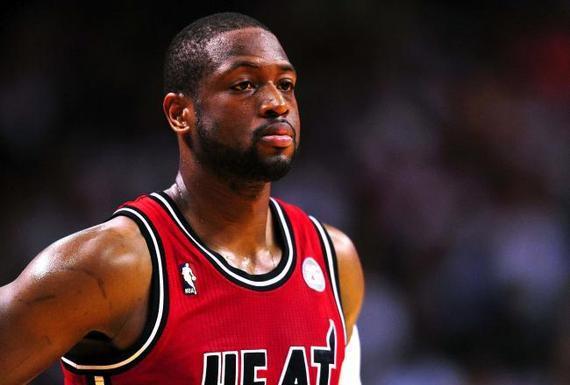
\includegraphics[width=5cm]{wade.jpg}\\
	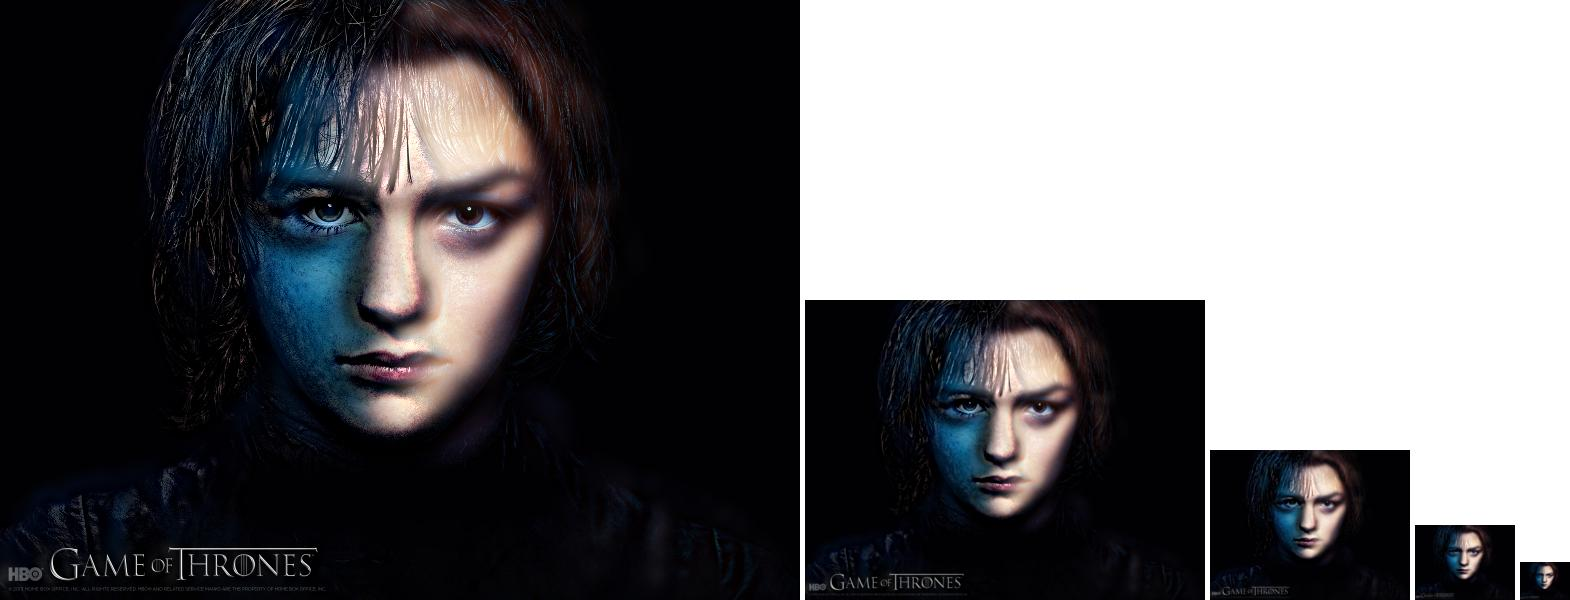
\includegraphics[width=10cm]{hybrid7.jpg}
	\caption{hybrid image 6}
\end{figure}
\newpage
\section{Speed Test}
I test the speed between direct 2D convolution and convolution through FFT. Clearly, the FFT is much faster in different sizes.
\begin{table}[h]
    \centering
    \begin{tabular}{lrrr}
       	\hline
        Image 	&Size 	&Method &Time(seconds) \\
        \hline
        1 		& 361$\times$410 	&Direct	&3.076361\\
         		&  &FFT	&0.053615\\
       	\hline
       	2 		& 331$\times$375 	&Direct	&1.528859\\
       	&  &FFT	&0.042454\\
       	\hline
       	3 		& 265$\times$225 	&Direct	&0.816425\\
       	&  &FFT	&0.022070\\
       	\hline
       	4 		& 300$\times$453 	&Direct	&1.907693\\
       	&  &FFT	&0.038621\\
       	\hline
       	5 		& 307$\times$375 	&Direct	&1.569954\\
       	&  &FFT	&0.038324\\
       	\hline
       	6 		& 450$\times$398 	&Direct	&2.573566\\
       	&  &FFT	&0.052624\\
       	\hline
    \end{tabular}
    \caption{Speed Test in different methods and sizes}
\end{table}
\section{Bouns}
	\begin{enumerate}
		\item Using reflected image content in the code(I called it symmetric padding).
		\item Using my own hybrid image in the result.
		\item Using FFT to process convolution in the code.
	\end{enumerate}
\section{Open question}
\begin{enumerate}
	\item The difference between different kinds of padding\\
	\textbf{My Idea:} When we handle the image edges during convolution, we need pad the matrix. Zero padding is obvious the nature way and easy to implement. But if we use zero padding, equivalently we add a black box outside the image. In some way, it looks like not very nature. So we have symmetric padding and cyclic padding. I think the former makes general images more smooth and the later is often used to cyclic image like regular vein.
	\newpage
	\item Scaling and Smoothing\\
	\textbf{My Idea:} As we all know, if we shrink a image to some extend, we will lack the precise information about object shapes or else details. Also, smoothing is dong the same thing. We ignore details and focus on object contours which is the information provided by low frequencies. So I try to use low pass filter that is gaussian filter to simulate the effect created by shrinking the hybrid image.
	\begin{figure}[h]
		\centering
		\includegraphics[width=7cm]{hybrid8.jpg}
		\caption{the result of filtering several times}
	\end{figure} 
\end{enumerate}
\end{document}